%\documentclass[notes]{beamer}       % print frame + notes
%\documentclass[notes=only]{beamer}   % only notes
\documentclass{beamer}              % only frames

\usetheme{Dresden}
\usecolortheme{orchid}
\usepackage{natbib}
\usepackage[export]{adjustbox}


% These are the configurable settings
% Please change them to make it fit your course
\def \institute {ErasmusMC}
\def \authors { Youri Hoogstrate, Saskia Hiltemann, David van Zessen, Andrew Stubbs}

\def \servers {
\begin{itemize}
	\item \url{https://bioinf-galaxian.erasmusmc.nl/galaxy/}
\end{itemize}
}
\def \datalibrarydirintroduction {
	EMC Training - Galaxy101
}

\def \datalibrarydirrnaseqtuxedo {
	EMC Galaxy Training Materials
		$\rightarrow$
	EMC Galaxy Training - 3: RNASeq Tuxedo Pipeline
}

\def \datalibrarydirrnaseqadvanced {
	EMC Galaxy Training Materials
		$\rightarrow$
	EMC Galaxy Training - 5: Advanced RNA-Seq Analysis
}

\tuxedofalse
% Configurations should be changed in this file


\title[Galaxy 101]{Galaxy 101}
\subtitle{Introduction to the Galaxy Project web platform}
%\author[\authors]
%\institute[\institutes]
\subject{Bioinformatics}


\setbeamercolor{footlinecolor}{fg=white,bg=UniBlue}
\makeatletter
\setbeamertemplate{footline}
{
\leavevmode%
\hbox{%
	\begin{beamercolorbox}[wd=.2\paperwidth,ht=0.6cm,left]{bg=white}
    		%\includegraphics[scale=0.3]{erasmusLogo.png}
  	\end{beamercolorbox}%
  	\begin{beamercolorbox}[wd=.6\paperwidth,ht=2.25ex,dp=1ex,center]{section in head/foot}%
    		\usebeamerfont{title,data}Introduction to Galaxy{ }{ }{ }\insertshortdate
  \end{beamercolorbox}%
  \begin{beamercolorbox}[wd=.2\paperwidth,ht=0.9cm,dp=1ex,center]{bg=white}%
    		%\includegraphics[scale=0.27]{trait.png}
  \end{beamercolorbox}}%
  \vskip0pt%
}
\makeatother

\begin{document}
\begin{frame}
	\titlepage % Print the title page as the first slide
\end{frame}

%\begin{frame}
%	\frametitle{Overview} % Table of contents slide, comment this block out to remove it
%	\begin{scriptsize}
%		\tableofcontents
%	\end{scriptsize}
%\end{frame}

\section{Introduction}

\subsection{What is Galaxy?}
\begin{frame}
    \frametitle{What is Galaxy?}
%    \framesubtitle{}
	Galaxy is an open, web-based platform for data intensive biomedical research.
	\begin{itemize}
		\item Provides graphical user interface for command-line programs
		\item Focus on \textbf{reproducibility} and high throughput sequencing
		\item User can build workflows graphically
		\item Analysis steps performed on datasets recorded in the \textbf{History}
		\item \textbf{Sharing} of datasets and workflows amongst users
		\item Free and open-source, large user/developer community
		\item Easy to run your own Galaxy instance
	\end{itemize}
	\begin{figure}
		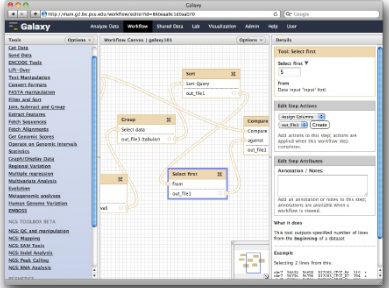
\includegraphics[height=0.25\textheight]{figures/101p_01a.png} \qquad\qquad
		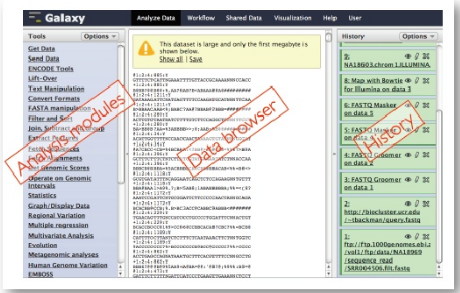
\includegraphics[height=0.25\textheight]{figures/101p_01b.png}
	\end{figure}
\end{frame}

\begin{frame}
    \frametitle{What is Galaxy?}
	\begin{figure}
		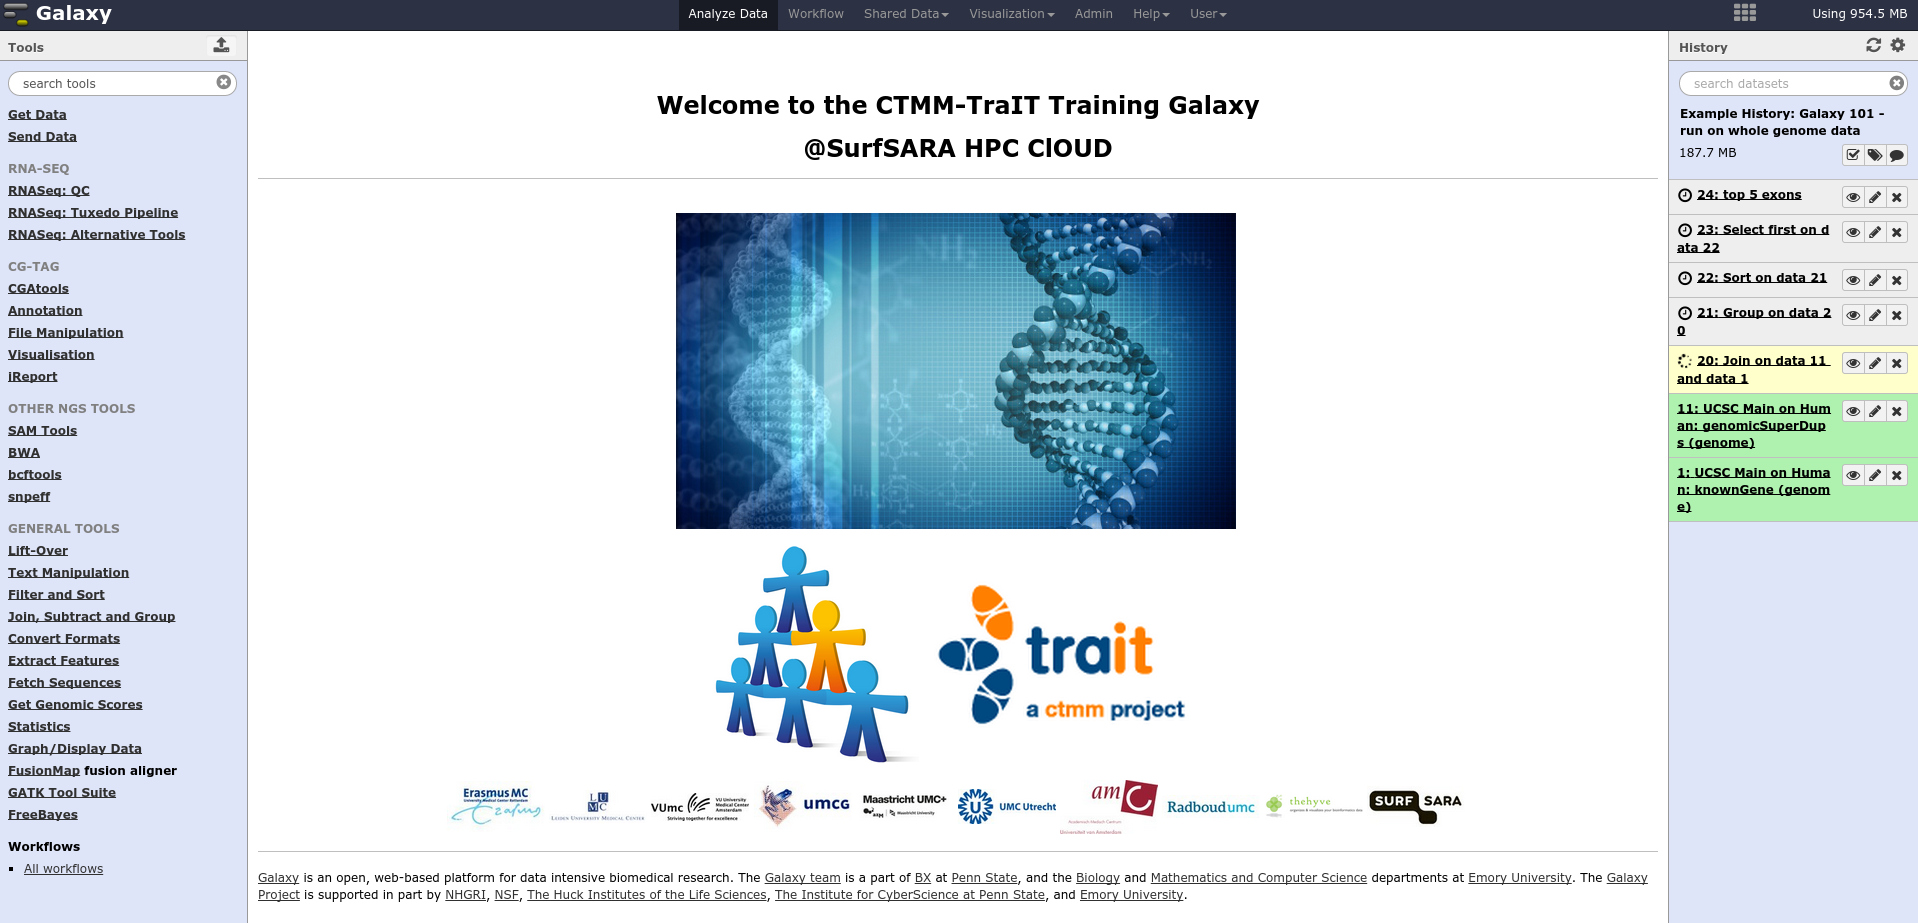
\includegraphics[width=\textwidth]{figures/101p_02.png}
	\end{figure}
\end{frame}

\subsection{Reproducibility}
\begin{frame}
    \frametitle{Reproducibility in Galaxy}
    \begin{itemize}
	    \item Every piece of data is read-only
	    \item Every tool has a version and modification dependent UID
	    \item Every tool or analysis does some operation or function on data, which will generate a \textbf{new} piece of read-only data
	    \item Each operation is a \textbf{step} between two or more pieces of data forming a modular workflow
	    \item Input data and the same workflow should produce the same outcome - also across different machines and OSes (\textbf{reproducible})
    	\begin{itemize}
	    	\item This is very hard if not impossible, but the closer the better
	    	\item Why is this complicated? Get exactly the same software (R versions, package versions, C library versions), compile them the same way (OS X / linux), 32/64bit, many factors in the entire chain
    	\end{itemize}
    \end{itemize}
\end{frame}

\section{Usage}
\subsection{Getting data}
\begin{frame}
    \frametitle{Getting data}
    \begin{itemize}
	    \item Upload via browser
	    \item Upload via FTP (for very large datasets)
	    \item Let Galaxy pull from external sources
	    \begin{itemize}
	    	\item UCSC
		    \item SRA
		    \item EBI
		    \item BioMart
		    \item \dots
	    \end{itemize}
    \end{itemize}
	\begin{figure}
		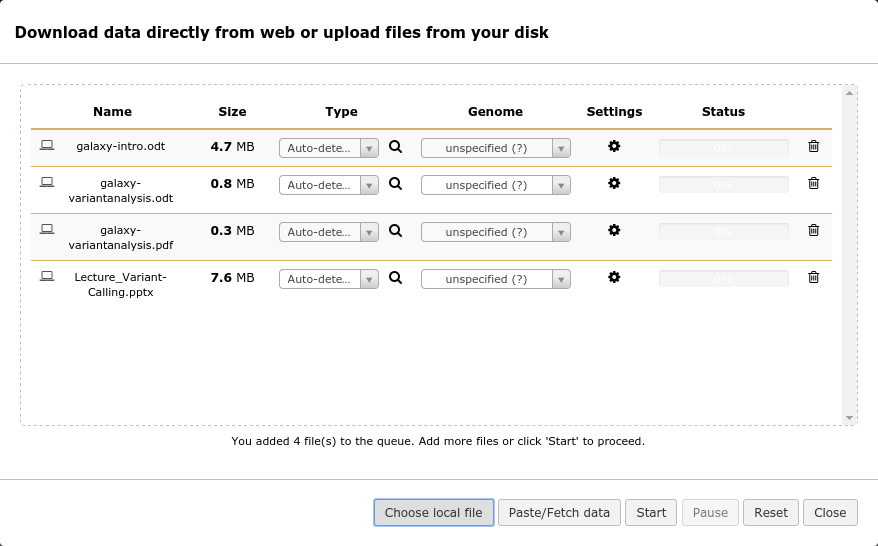
\includegraphics[width=0.5\textwidth,left]{figures/101p_03.png}
	\end{figure}
\end{frame}

\subsection{Histories}
\begin{frame}
\frametitle{Histories}
  \begin{columns}[T]
    \begin{column}{.82\textwidth}
	\begin{itemize}
	\item Items coloured by status:
		\begin{itemize}
		\item Green: completed successfully
		\item Yellow: running {\scriptsize \textbf{*}}
		\item Grey: queued {\scriptsize \textbf{*}}
		\item Red: completed with error
		\end{itemize}
	\item Buttons:
		\begin{itemize}
		\item Eye: view contents of file
		\item Pencil: edit attributes (name, reference genome, file type, convert format, etc..)
		\end{itemize}
	\end{itemize}
    \end{column}
    \begin{column}{.18\textwidth}
		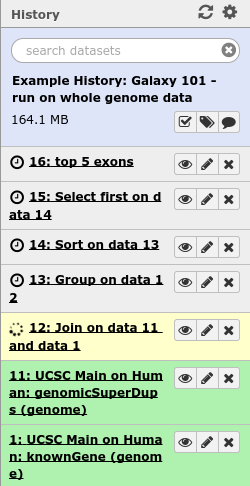
\includegraphics[width=\textwidth,right]{figures/101p_04a.png}
    \end{column}
  \end{columns}
  \ \\
  \ \\
  {\scriptsize \textbf{*May take a while, be patient, grab a coffee, do not spawn duplicate jobs!}}
\end{frame}

\begin{frame}
\frametitle{Histories}
  \begin{columns}[T]
    \begin{column}{.82\textwidth}
	\begin{itemize}
	\item Expand history item for more options
		\begin{itemize}
		\item Download
		\item View metadata
		\item View output/error logs
		\item Visualisation options
		\item Rerun tool
		\end{itemize}
	\item Metadata is recorded:
		\begin{itemize}
		\item Tool versions
		\item Reference genome
		\item Full parameter settings
		\item Input files used
		\end{itemize}
	\end{itemize}
    \end{column}
    \begin{column}{.18\textwidth}
		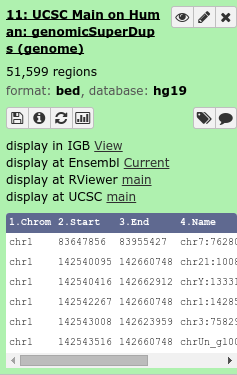
\includegraphics[width=\textwidth,right]{figures/101p_04b.png}
    \end{column}
  \end{columns}
\end{frame}
	

\subsection{Visualizations}
\begin{frame}
\frametitle{Visualizations}
  \begin{columns}[T]
    \begin{column}{.72\textwidth}
	\begin{itemize}
	\item Built-in interactive visualizations:
		\begin{itemize}
		\item Genome browser: Trackster
		\item Circos-like views with Circster
		\item Custom plots with Galaxy Charts
		\end{itemize}
	\item Links to external display applications:
		\begin{itemize}
			\item UCSC
 			\item IGV, IGB
 			\item Ensemble
 			\item \ldots
		\end{itemize}
		\item Visualization tools:
		\begin{itemize}
			\item JBrowse
 			\item iReport
 			\item \ldots
		\end{itemize}
	\end{itemize}
    \end{column}
    \begin{column}{.28\textwidth}
		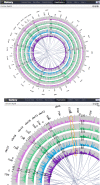
\includegraphics[width=\textwidth,right]{figures/101p_06.png}
    \end{column}
  \end{columns}
\end{frame}

\subsection{Sharing}
\begin{frame}
\frametitle{Sharing}
  \begin{columns}[T]
    \begin{column}{.72\textwidth}
	\begin{itemize}
	\item \textbf{Data Libraries: } admins make data libraries available to share often-used data with all users.
	\item \textbf{Histories, workflows, visualisations: } Users can share their work by:
		\begin{itemize}
		\item Sharing with specific Galaxy users
		\item Make accessible via link. Anybody with this link can see
	   your shared data (even without an account)
		\item Publishing on Galaxy (will appear in shared data menu and as perma-link)
		\end{itemize}
	\item \textbf{Published Pages} Virtual manual pages containing \textbf{all} elements of galaxy
	\end{itemize}
    \end{column}
    \begin{column}{.28\textwidth}
		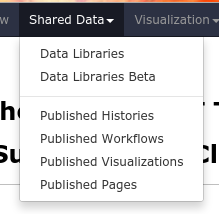
\includegraphics[width=\textwidth,right]{figures/101p_07.png}
    \end{column}
  \end{columns}
\end{frame}

\begin{frame}
	\frametitle{Sharing: published pages}
	\begin{figure}
		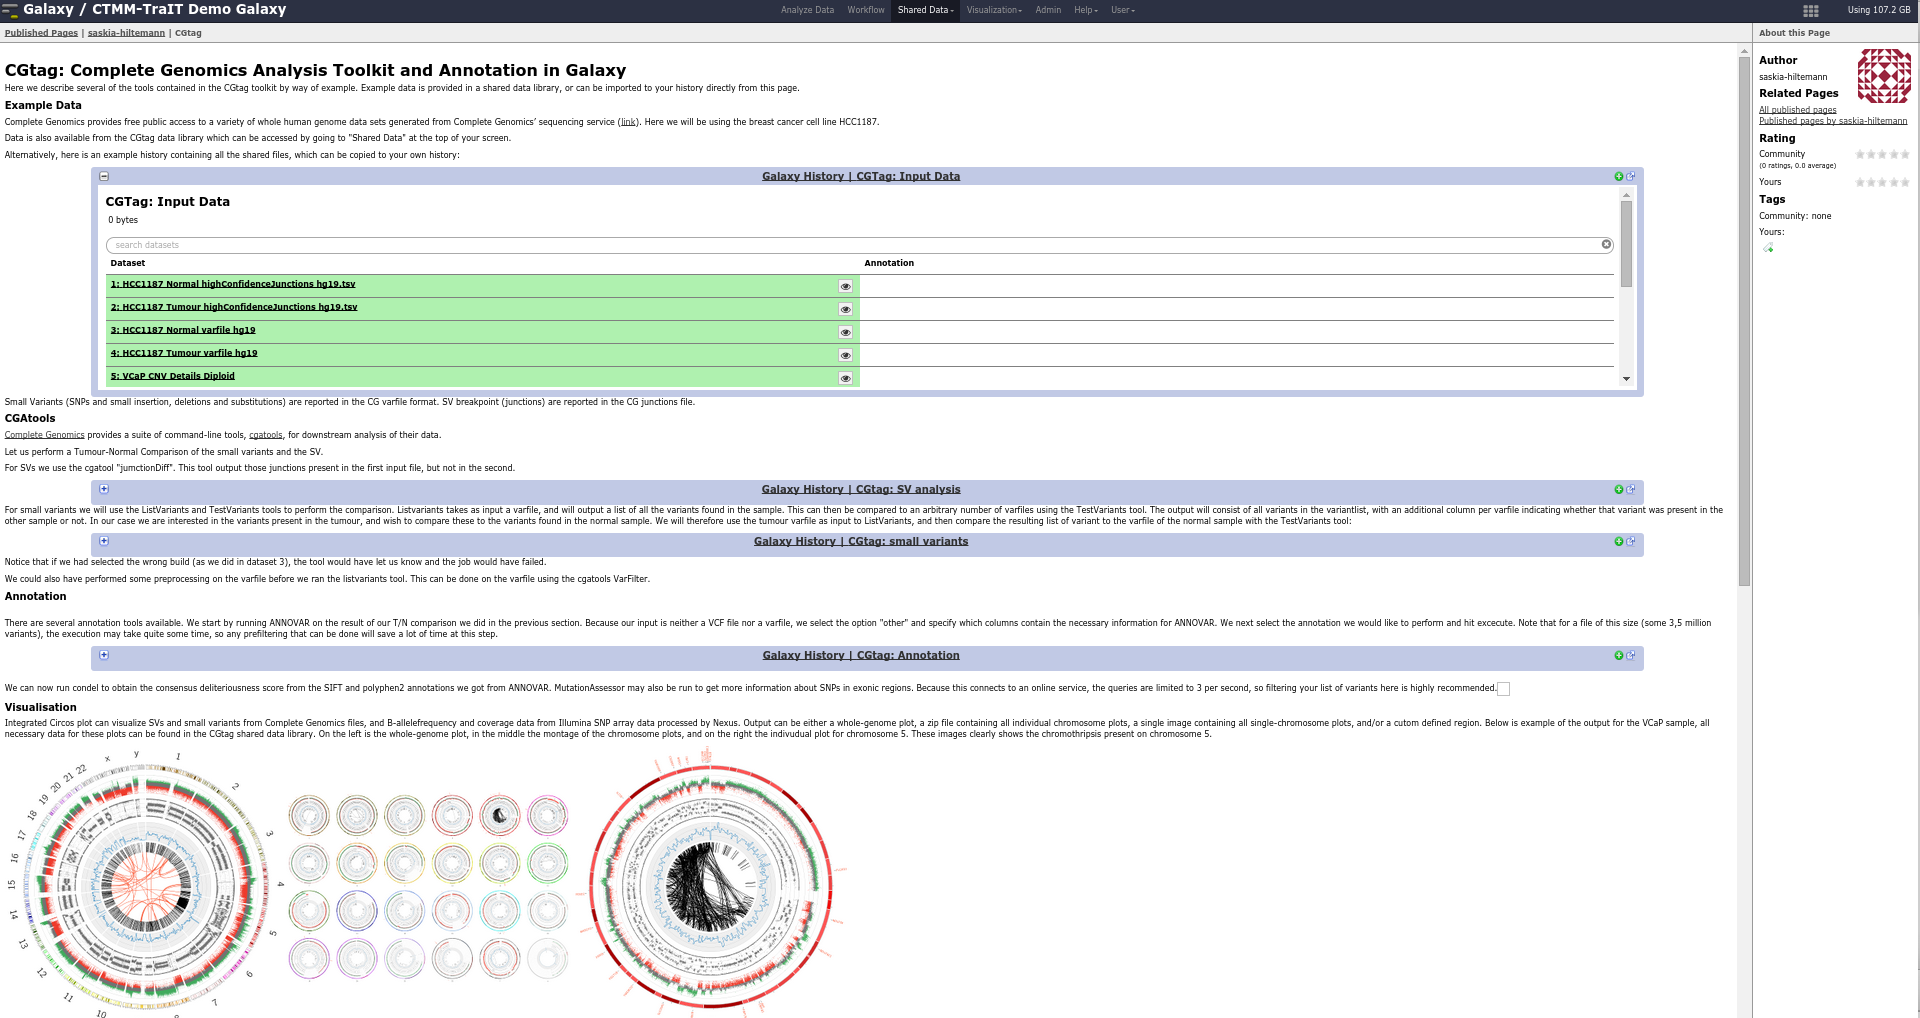
\includegraphics[width=\textwidth]{figures/101p_08.png}
	\end{figure}
\end{frame}

\section{Advanced}
\begin{frame}
\frametitle{Advanced topics}
  \begin{columns}[T]
    \begin{column}{.82\textwidth}
	\begin{itemize}
	\item \textbf{Tool Shed} The Bioinformatics App Store
		\begin{itemize}
		\item 3000+ tools (C, Per, Python, Bash, JS, etc. etc.)
		\item Dependency management
		\item Data managers - build and manage reference genomes (and indices for tools)
		\end{itemize}
	\item \textbf{API} 	Programmatic (automated) access to Galaxy	
		\begin{itemize}
			\item Example: embbed galaxy tools into other workflow systems
		\end{itemize}
	\end{itemize}
    \end{column}
    \begin{column}{.18\textwidth}
		
\includegraphics[width=\textwidth,right]{figures/101p_09.jpg}
    \end{column}
  \end{columns}
\end{frame}

\section*{Preparations}
\subsection*{Open Galaxy}
\begin{frame}
\frametitle{Preparation}
Obtain the course manual (module Galaxy101) from:
\begin{itemize}
	\item \url{https://bioinf-galaxian.erasmusmc.nl/public/GalaxyTraining/EMC2016/}
\end{itemize}

\ \\
Open a web browser and navigate to the Galaxy server:
\servers
\ \\
and follow the instructions in the course manual.
\end{frame}
% Preparations should describe how to access which server



%\note{Note}

%\section{References}
%\begin{frame}[allowframebreaks]
%\frametitle{References}
%\bibliographystyle{plain}
%\begin{tiny}
%	\bibliography{references}
%\end{tiny}
%\end{frame}

\end{document}
